\documentclass[12pt,a4paper,openright,final]{article}
\usepackage{fontspec}
\usepackage{amsmath}
\usepackage{amsfonts}
\usepackage{amssymb}
\usepackage{makeidx}
\usepackage{graphicx}
\usepackage[hidelinks,unicode=true]{hyperref}
\usepackage[spanish,es-nodecimaldot,es-lcroman,es-tabla,es-noshorthands]{babel}
\usepackage[left=3cm,right=2cm, bottom=4cm]{geometry}
\usepackage{natbib}
\usepackage{microtype}
\usepackage{ifdraft}
\usepackage{verbatim}
\usepackage[obeyDraft]{todonotes}
\ifdraft{
	\usepackage{draftwatermark}
	\SetWatermarkText{BORRADOR}
	\SetWatermarkScale{0.7}
	\SetWatermarkColor{red}
}{}
\usepackage{booktabs}
\usepackage{longtable}
\usepackage{calc}
\usepackage{array}
\usepackage{caption}
\usepackage{subfigure}
\usepackage{footnote}
\usepackage{url}
\usepackage{tikz}

\setsansfont[Ligatures=TeX]{texgyreadventor}
\setmainfont[Ligatures=TeX]{texgyrepagella}

\author{José Ignacio Escribano}

%*******************************************************
%                 NO MODIFICAR
\newcommand*{\FSfont}[1]{%
  \fontencoding{T1}\fontfamily{#1}\selectfont}

\newlength{\tpheight}\setlength{\tpheight}{0.9\textheight}
\newlength{\txtheight}\setlength{\txtheight}{0.9\tpheight}
\newlength{\tpwidth}\setlength{\tpwidth}{0.9\textwidth}
\newlength{\txtwidth}\setlength{\txtwidth}{0.9\tpwidth}
\newlength{\drop}
%*******************************************************

% Crea una portada con los siguientes parámetros
%
% #1 : Título 
% #2 : Subtítulo
% #3 : Subsubtítulo
% #4 : Autor(es)
% #5 : Lugar
%

\newcommand*{\portada}[5]{
\begin{titlepage}
\begingroup
\vspace*{1cm}
\drop = 0.2\txtheight
\centering
\vfill
{\Huge \scshape #1}\\[\baselineskip]
{\Large \textbf{#2}}\\[\baselineskip]
{\Large \scshape #3}\\[\baselineskip]
\vspace*{0.3cm}
{\large \textit{#4}}\\[0.5\drop]

\includegraphics[scale=0.35]{./imagenes/logoURJC.jpg}
\vspace*{1.5cm}

{\large \scshape #5, \today} \par
\begin{center}
\end{center}
\vfill\null
\endgroup
\end{titlepage}
}
 %*****************************************************
 


\title{Actividad II. Ingeniería de la Decisión \\ \textbf{Resolución de un problema de decisión con GeNIe}}

\setlength{\parindent}{0pt}

\begin{document}

\portada{Actividad II}{Ingeniería de la Decisión}{Resolución de un problema de decisión con GeNIe}{José Ignacio Escribano}{Móstoles}

\listoffigures
\thispagestyle{empty}
\newpage

\listoftables
\thispagestyle{empty}
\newpage

\tableofcontents
\thispagestyle{empty}
\newpage

\pagenumbering{arabic}
\setcounter{page}{1}

\section{Introducción}

Se le presenta la oportunidad de adquirir una opción del Gobierno cubano para explotar un pozo de petróleo de 5.000.000 de barriles a 5 € por barril. Repsol cree que después de procesamiento, transporte y refino, puede obtener 8 € por barril en el mercado USA. Sin embargo, a consecuencia de la ley Helms-Burton, Repsol teme no recibir autorización del gobierno USA, con lo que debería pagar una multa a Cuba de 1€ por barril, por no hacer efectiva la operación. Repsol estima que hay probabilidad 0.7 de no recibir la autorización para la importación si gana el Partido Republicano en el Congreso  y 0.4 si gana el Partido Demócrata. En estos momentos, NYT da ganador al Partido Republicano con probabilidad 0.56.\\

Para reducir su incertidumbre, estudia contratar a Arnald’s, un bufete que puede estudiar en detalle el caso por 100.000 €, y puede hacer un informe ``Favorable'' o ``Desfavorable''. Según el dossier que presenta Arnald’s, de 20 ocasiones previas que se consiguió la autorización, en 19 emitió informe ``Favorable''. Igualmente, indican que en 10 ocasiones en que no se recibió la autorización, habían emitido informe favorable en 3 de ellas.\\
 
Determinar si merece o no la pena contratar a Arnald’s, y si Repsol debe ejercer o no la opción, resolviendo el  diagrama de influencia del problema con GeNIe.

\section{Resolución del problema}

Para resolver el problema, seguimos las fases del ciclo de análisis de decisión: estructuración del problema, modelización de creencias y preferencias y optimización.

\subsection{Estructuración del problema}
 
En primer lugar, identificamos los objetivos, incertidumbres del problema y las decisiones que debe tomar Repsol. En la Tabla~\ref{tbl:decisiones} se muestran los objetivos, las incertidumbres y decisiones del problema.\\

\begin{table}[htbp!]
	\centering
	\caption{Objetivos, incertidumbres y decisiones del problema}
	\label{tbl:decisiones}
	\begin{tabular}{@{}ccc@{}}
		\toprule
		\textbf{Objetivos}                                              & \textbf{Incertidumbres}                                                                                   & \textbf{Decisiones}                                                                      \\ \midrule
		\begin{tabular}[c]{@{}c@{}}Maximizar \\ beneficios\end{tabular} & \begin{tabular}[c]{@{}c@{}}Ganador de las elecciones según \\ la encuesta del New York Times\end{tabular} & Explotar o no el pozo                                                                    \\ \midrule
		& Recibir la autorización                                                                                   & \begin{tabular}[c]{@{}c@{}}Contratar o no al bufete \\ de abogados Arnald's\end{tabular} \\ \midrule
		\multicolumn{1}{l}{}                                            & Resultado del informe de Arnald's                                                                         & \multicolumn{1}{l}{}                                                                     \\ \bottomrule
	\end{tabular}
\end{table}

Una vez que tenemos identificados los elementos del problema, podemos crear el diagrama de influencia. Éste se muestra en la Figura~\ref{fig:diagrama_influencia}. Los estados de cada incertidumbre y las elecciones de las decisiones se muestran en la Tabla~\ref{tbl:estados}.

\begin{figure}[tbph!]
	\centering
	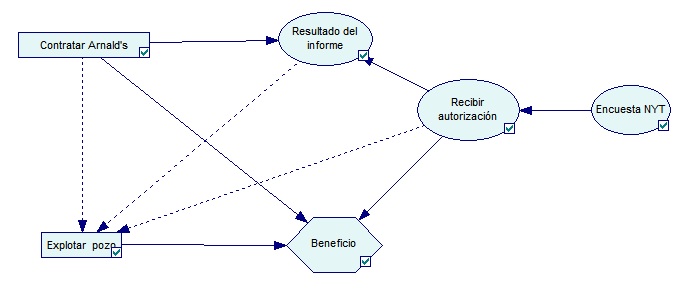
\includegraphics[width=\linewidth]{imagenes/diagrama_influencia.png}
	\caption{Diagrama de influencia del problema}
	\label{fig:diagrama_influencia}
\end{figure}

\begin{table}[htbp!]
	\centering
	\caption{Estados de las incertidumbres y elecciones de las decisiones del problema}
	\label{tbl:estados}
\resizebox{\textwidth}{!}{%
	\begin{tabular}{@{}cccccc@{}}
		\cmidrule(l){2-6}
		& \multicolumn{3}{c}{\textbf{Incertidumbres}}                                                                                                                                                                                                                         & \multicolumn{2}{c}{\textbf{Decisiones}}                                                                                           \\ \midrule
		& \begin{tabular}[c]{@{}c@{}}Ganador \\ de las elecciones\end{tabular}            & \begin{tabular}[c]{@{}c@{}}Recibir \\ la autorización\end{tabular} & \begin{tabular}[c]{@{}c@{}}Resultado \\ del informe\end{tabular}                                             & Explotar el pozo                                               & Contratar a Arnald's                                             \\ \midrule
		\begin{tabular}[c]{@{}c@{}}Estados/\\ Alternativas\end{tabular} & \begin{tabular}[c]{@{}c@{}}Partido Republicano\\ Partido Demócrata\end{tabular} & \begin{tabular}[c]{@{}c@{}}Recibir\\ No recibir\end{tabular}       & \begin{tabular}[c]{@{}c@{}}Favorable\\ Desfavorable\\ No hacer (si no \\ se contrata al bufete)\end{tabular} & \begin{tabular}[c]{@{}c@{}}Explotar\\ No explotar\end{tabular} & \begin{tabular}[c]{@{}c@{}}Contratar\\ No contratar\end{tabular} \\ \bottomrule
	\end{tabular}
}
\end{table}

Una vez que se conocen los estados de los nodos, los introducimos en GeNIe.

\subsection{Modelización de creencias}

Teniendo en cuenta los datos del enunciado se introducen las probabilidades de los nodos de azar en GeNIe, que se muestran en la Figura~\ref{fig:azar}.

\begin{figure}[htbp!]
	\centering
	\subfigure[Probabilidades del nodo Encuesta NYT]{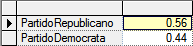
\includegraphics[width=0.45\linewidth]{./imagenes/nyt}}\hspace{10mm}
	\subfigure[Probabilidades del nodo Recibir autorización]{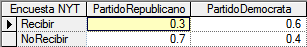
\includegraphics[width=0.45\linewidth]{./imagenes/autorizacion}}\vspace{10mm}
	\subfigure[Probabilidades del nodo Resultado informe]{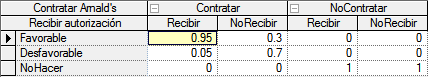
\includegraphics[width=0.9\linewidth]{./imagenes/resultado_informe}}
	\caption{Probabilidades de los nodos de azar} \label{fig:azar}
\end{figure}

\subsection{Optimización}

Para resolver el problema, sólo nos queda introducir la utilidad del nodo Beneficio. Para ello, calculamos el beneficio (en millones de euros) en cada uno de los posibles escenarios, es decir, todas las combinaciones de los estados de los nodos Contratar Arnald's, Recibir autorización y Explotar pozo (Figura~\ref{fig:utilidad}).\\

\begin{figure}[tbph!]
	\centering
	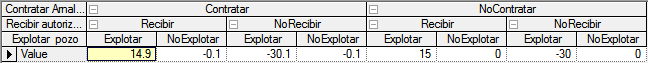
\includegraphics[width=\linewidth]{imagenes/utilidad.png}
	\caption{Utilidad del nodo Beneficio}
	\label{fig:utilidad}
\end{figure}

Calculemos algún escenario a modo de ejemplo. La utilidad de explotar el pozo, sabiendo que hemos recibido la autorización y hemos contratado a Arnald's es -0.1 (por contratar a Arnald's) -5*5 (por explotar el pozo) + 8*5 (por vender en el mercado USA) = 14.9 millones de euros.\\

La utilidad de explotar el pozo sabiendo que no hemos recibido la autorización y habiendo contratado a Arnald's es -0.1 (por contratar a Arnald's) -5*5 (por explotar el pozo) - 1*5 (multa de Cuba por no tener la autorización) = -30.1 millones de euros.\\

De forma similar se obtiene el resto de los casos.\\

Para finalizar, resolvemos el modelo con GeNIE para obtener los resultados. Los resultados (Figura~\ref{fig:resultado}) que se obtienen son los siguientes:\\

\begin{figure}[tbph!]
	\centering
	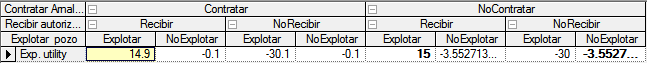
\includegraphics[width=\linewidth]{imagenes/resultado.png}
	\caption{Resultados del modelo}
	\label{fig:resultado}
\end{figure}

Observamos que la máxima utilidad esperada se obtiene cuando se decide no contratar a Arnald's, se recibe la autorización y se explota el pozo.\\

Si observamos los resultados del nodo Contratar Arnald's, la utilidad de Contratar es 6.38 y 6.48 para NoContratar. Por lo que no debemos contratar a este bufete de abogados.\\

Si ahora observamos los resultados del nodo Explotar pozo, observamos que tanto si contratamos como si no contratamos a Arnald's, la mejor opción es explotar el pozo si recibimos la autorización, y no explotar en caso de no recibirla, aunque el de máxima utilidad será cuando no se le contrate.\\

\begin{figure}[tbph!]
	\centering
	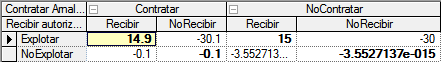
\includegraphics[width=\linewidth]{imagenes/resultados_pozo.png}
	\caption{Resultados del nodo Explotar pozo}
	\label{fig:resultados_pozo}
\end{figure}

En definitiva, para obtener la máxima utilidad, deberemos no contratar al bufete de abogados Arnald's, y explotar el pozo en caso de obtener la autorización, y no explotar si no obtenemos la autorización.\\

Si ahora la probabilidad de que gane el partido Republicano es de 0.4, debemos cambiar las probabilidades del nodo Encuesta NYT en el modelo de GeNIe. Si resolvemos el diagrama de influencia, tenemos el mismo resultado global anterior, pero con utilidades diferentes. En el caso del nodo Contratar Arnald's tenemos una utilidad de 7.2 para no contratar, por 7.1 para contratar. En el caso del nodo de Explotar pozo, se obtienen los mismos resultados que en el caso anterior.\\

Si, por último, consideramos que la probabilidad de que gane el partido Republicano es de 0.8, los resultados son idénticos al caso anterior: sólo varía la utilidad de contratar a Arnald's: 5.4 en caso de no contratar, por 5.3 en caso de contratar.\\

A tenor de los resultados, parece que el partido que gane las elecciones no tiene demasiada importancia en el resultado de nuestra elección.

\subsection{Conclusiones}

En definitiva, no debemos contratar al bufete de abogados Arnald's. En caso de recibir la autorización debemos explotar el pozo, y si no la recibimos, no explotar el pozo.\\

También, hemos comprobado que el resultado del ganador de las elecciones según el New York Times, no condiciona el resultado del problema: debemos tomar las mismas decisiones, aunque la utilidad esperada no es igual según la probabilidad de que gane un partido u otro.

\section{Conclusiones}

En esta actividad, hemos puesto en conjunto todo el ciclo de análisis de decisiones: desde la estructuración del problema hasta la optimización (faltaría hacer un análisis de sensibilidad) para resolver un problema real  (aunque simplificado) de toma de decisiones. Para resolverlo, hemos utilizado el software GeNIe que de forma sencilla permite la creación, edición y resolución de diagramas de influencia, ahorrando una gran cantidad de tiempo.

\end{document} 